% Options for packages loaded elsewhere
\PassOptionsToPackage{unicode}{hyperref}
\PassOptionsToPackage{hyphens}{url}
%
\documentclass[
  12pt,
  a4paper,
  DIV=11,
  numbers=noendperiod]{scrreprt}

\usepackage{amsmath,amssymb}
\usepackage{setspace}
\usepackage{iftex}
\ifPDFTeX
  \usepackage[T1]{fontenc}
  \usepackage[utf8]{inputenc}
  \usepackage{textcomp} % provide euro and other symbols
\else % if luatex or xetex
  \usepackage{unicode-math}
  \defaultfontfeatures{Scale=MatchLowercase}
  \defaultfontfeatures[\rmfamily]{Ligatures=TeX,Scale=1}
\fi
\usepackage{lmodern}
\ifPDFTeX\else  
    % xetex/luatex font selection
\fi
% Use upquote if available, for straight quotes in verbatim environments
\IfFileExists{upquote.sty}{\usepackage{upquote}}{}
\IfFileExists{microtype.sty}{% use microtype if available
  \usepackage[]{microtype}
  \UseMicrotypeSet[protrusion]{basicmath} % disable protrusion for tt fonts
}{}
\usepackage{xcolor}
\setlength{\emergencystretch}{3em} % prevent overfull lines
\setcounter{secnumdepth}{5}
% Make \paragraph and \subparagraph free-standing
\ifx\paragraph\undefined\else
  \let\oldparagraph\paragraph
  \renewcommand{\paragraph}[1]{\oldparagraph{#1}\mbox{}}
\fi
\ifx\subparagraph\undefined\else
  \let\oldsubparagraph\subparagraph
  \renewcommand{\subparagraph}[1]{\oldsubparagraph{#1}\mbox{}}
\fi


\providecommand{\tightlist}{%
  \setlength{\itemsep}{0pt}\setlength{\parskip}{0pt}}\usepackage{longtable,booktabs,array}
\usepackage{calc} % for calculating minipage widths
% Correct order of tables after \paragraph or \subparagraph
\usepackage{etoolbox}
\makeatletter
\patchcmd\longtable{\par}{\if@noskipsec\mbox{}\fi\par}{}{}
\makeatother
% Allow footnotes in longtable head/foot
\IfFileExists{footnotehyper.sty}{\usepackage{footnotehyper}}{\usepackage{footnote}}
\makesavenoteenv{longtable}
\usepackage{graphicx}
\makeatletter
\def\maxwidth{\ifdim\Gin@nat@width>\linewidth\linewidth\else\Gin@nat@width\fi}
\def\maxheight{\ifdim\Gin@nat@height>\textheight\textheight\else\Gin@nat@height\fi}
\makeatother
% Scale images if necessary, so that they will not overflow the page
% margins by default, and it is still possible to overwrite the defaults
% using explicit options in \includegraphics[width, height, ...]{}
\setkeys{Gin}{width=\maxwidth,height=\maxheight,keepaspectratio}
% Set default figure placement to htbp
\makeatletter
\def\fps@figure{htbp}
\makeatother

\KOMAoption{captions}{tableheading}
\usepackage{indentfirst}
\usepackage{float}
\floatplacement{figure}{H}
\usepackage[math,RM={Scale=0.94},SS={Scale=0.94},SScon={Scale=0.94},TT={Scale=MatchLowercase,FakeStretch=0.9},DefaultFeatures={Ligatures=Common}]{plex-otf}
\makeatletter
\@ifpackageloaded{caption}{}{\usepackage{caption}}
\AtBeginDocument{%
\ifdefined\contentsname
  \renewcommand*\contentsname{Содержание}
\else
  \newcommand\contentsname{Содержание}
\fi
\ifdefined\listfigurename
  \renewcommand*\listfigurename{Список иллюстраций}
\else
  \newcommand\listfigurename{Список иллюстраций}
\fi
\ifdefined\listtablename
  \renewcommand*\listtablename{Список таблиц}
\else
  \newcommand\listtablename{Список таблиц}
\fi
\ifdefined\figurename
  \renewcommand*\figurename{Рисунок}
\else
  \newcommand\figurename{Рисунок}
\fi
\ifdefined\tablename
  \renewcommand*\tablename{Таблица}
\else
  \newcommand\tablename{Таблица}
\fi
}
\@ifpackageloaded{float}{}{\usepackage{float}}
\floatstyle{ruled}
\@ifundefined{c@chapter}{\newfloat{codelisting}{h}{lop}}{\newfloat{codelisting}{h}{lop}[chapter]}
\floatname{codelisting}{Список}
\newcommand*\listoflistings{\listof{codelisting}{Листинги}}
\makeatother
\makeatletter
\makeatother
\makeatletter
\@ifpackageloaded{caption}{}{\usepackage{caption}}
\@ifpackageloaded{subcaption}{}{\usepackage{subcaption}}
\makeatother
\ifLuaTeX
\usepackage[bidi=basic]{babel}
\else
\usepackage[bidi=default]{babel}
\fi
\babelprovide[main,import]{russian}
\babelprovide[import]{english}
% get rid of language-specific shorthands (see #6817):
\let\LanguageShortHands\languageshorthands
\def\languageshorthands#1{}
\ifLuaTeX
  \usepackage{selnolig}  % disable illegal ligatures
\fi
\usepackage[style=gost-numeric,backend=biber,langhook=extras,autolang=other*]{biblatex}
\addbibresource{bib/cite.bib}
\usepackage{csquotes}
\usepackage{bookmark}

\IfFileExists{xurl.sty}{\usepackage{xurl}}{} % add URL line breaks if available
\urlstyle{same} % disable monospaced font for URLs
\hypersetup{
  pdftitle={Отчет по лабораторной работе 2},
  pdfauthor={Власов Артем Сергеевич},
  pdflang={ru-RU},
  hidelinks,
  pdfcreator={LaTeX via pandoc}}

\title{Отчет по лабораторной работе 2}
\usepackage{etoolbox}
\makeatletter
\providecommand{\subtitle}[1]{% add subtitle to \maketitle
  \apptocmd{\@title}{\par {\large #1 \par}}{}{}
}
\makeatother
\subtitle{Власов Артем Сергеевич}
\author{Власов Артем Сергеевич}
\date{}

\begin{document}
\maketitle

\renewcommand*\contentsname{Содержание}
{
\setcounter{tocdepth}{1}
\tableofcontents
}
\listoffigures
\listoftables
\setstretch{1.5}
\chapter{Цель
работы}\label{ux446ux435ux43bux44c-ux440ux430ux431ux43eux442ux44b}

Выполнить действия по созданию и управлению групп и учетных записей
пользователей с помощью командной строки.

\chapter{Задание}\label{ux437ux430ux434ux430ux43dux438ux435}

Научиться создавать новые учетные записи и группы, добавлять учетные
записи в группы, задавать им определенные права, ответить на контрольные
вопросы.

\chapter{Выполнение лабораторной работы
2.}\label{ux432ux44bux43fux43eux43bux43dux435ux43dux438ux435-ux43bux430ux431ux43eux440ux430ux442ux43eux440ux43dux43eux439-ux440ux430ux431ux43eux442ux44b-2.}

Получим информацию о нашем пользователе.

\begin{figure}

{\centering 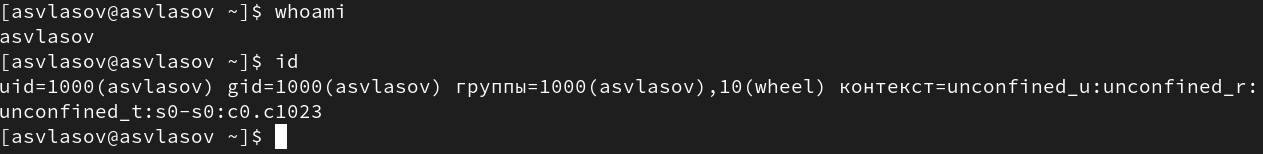
\includegraphics[width=0.7\textwidth,height=\textheight]{image/1.png}

}

\caption{Пользователь}

\end{figure}%

whoami показывает имя учетной записи пользователя, id показывает uid
пользователя, его номер в системе, и группы в которых он состоит.

Посмотрим информацию о root учетной записи.

\begin{figure}

{\centering 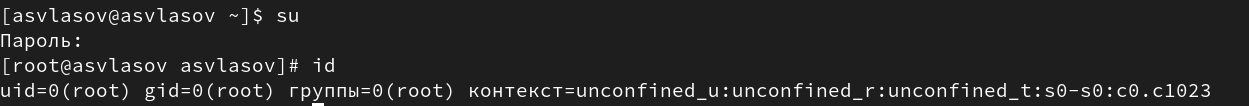
\includegraphics[width=0.7\textwidth,height=\textheight]{image/2.png}

}

\caption{Рут}

\end{figure}%

Номер пользователя 0, состоит в группе root. Обладает правами
суперпользователя.

Проверяем строчку wheel в файле.

\begin{figure}

{\centering 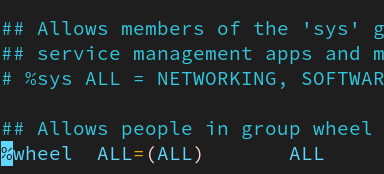
\includegraphics[width=0.7\textwidth,height=\textheight]{image/3.png}

}

\caption{wheel}

\end{figure}%

Группа wheel это группа пользователей с правами администратора системы.

Создаем пользователя alice и сразу добавляем его в группу
администраторов, задаем пароль для учетной записи.

\begin{figure}

{\centering 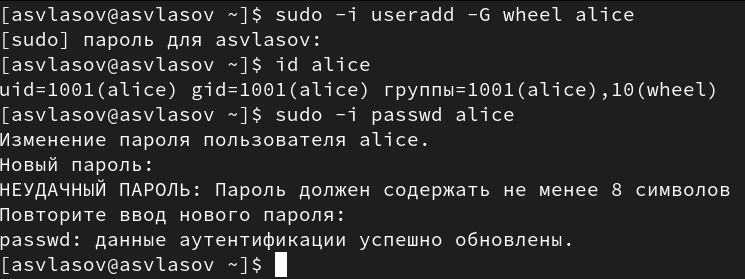
\includegraphics[width=0.7\textwidth,height=\textheight]{image/4.png}

}

\caption{Новый пользователь}

\end{figure}%

Переключаемся на пользователя администратора aliceи создаем нового
пользователя bob.

\begin{figure}

{\centering 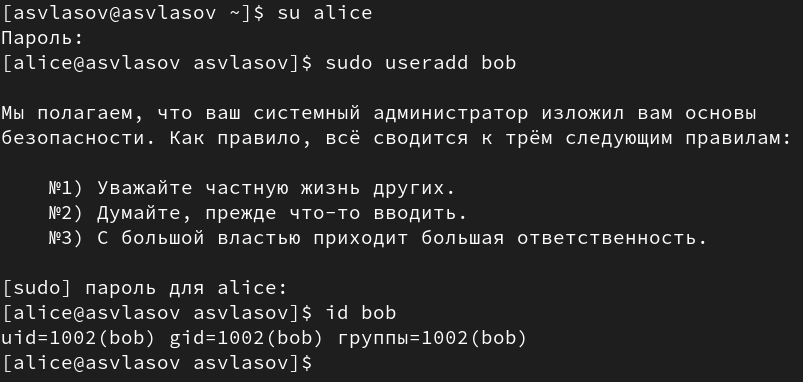
\includegraphics[width=0.7\textwidth,height=\textheight]{image/5.png}

}

\caption{БОБ}

\end{figure}%

Проверяем и изменяем настройки в файле bashrc.

\begin{figure}

{\centering 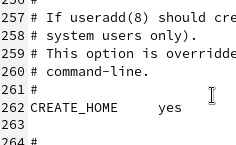
\includegraphics[width=0.7\textwidth,height=\textheight]{image/6.png}

}

\caption{1}

\end{figure}%%
\begin{figure}

{\centering 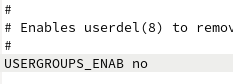
\includegraphics[width=0.7\textwidth,height=\textheight]{image/7.png}

}

\caption{2}

\end{figure}%

Добавляем в папку skel директории картинок и документов, чтобы они были
у каждого нового пользователя.

\begin{figure}

{\centering 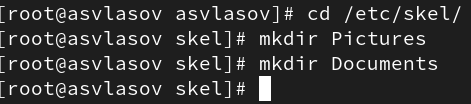
\includegraphics[width=0.7\textwidth,height=\textheight]{image/8.png}

}

\caption{Добавление директорий}

\end{figure}%

Задаем gedit, как редактор файлов по умолчанию.

\begin{figure}

{\centering 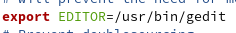
\includegraphics[width=0.7\textwidth,height=\textheight]{image/9.png}

}

\caption{гедит}

\end{figure}%

Создаем нового пользователя carol и задаем ему пароль.

\begin{figure}

{\centering 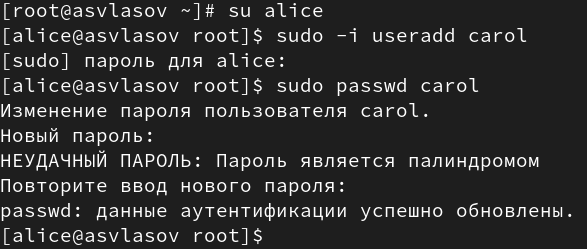
\includegraphics[width=0.7\textwidth,height=\textheight]{image/10.png}

}

\caption{Новый пользовательь}

\end{figure}%

Переходим в нового пользователя, и читаем информацию о нем.

\begin{figure}

{\centering 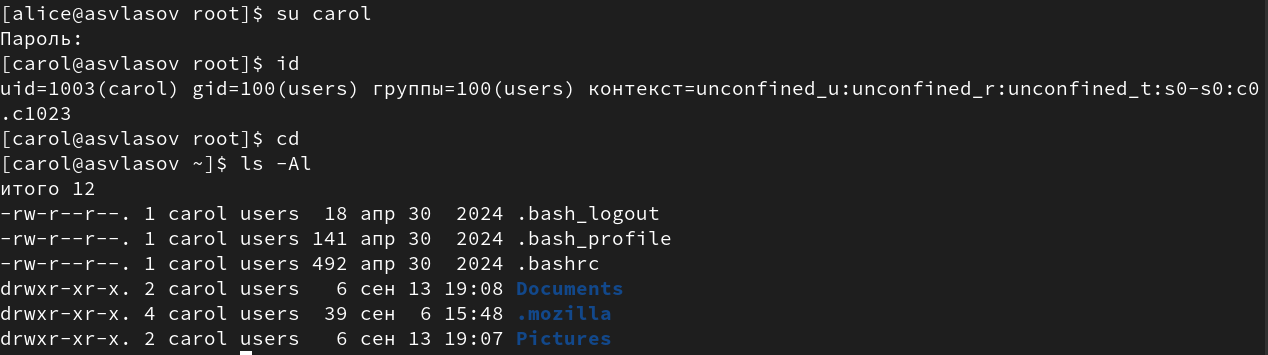
\includegraphics[width=0.7\textwidth,height=\textheight]{image/11.png}

}

\caption{Информация пользователя}

\end{figure}%

Видим, что пользователь имеет 3 номер, и находится в группе user, так же
проверяем, что профиль файла bashrc и директории обновились для каждого
нового пользователя.

Смотрим пароль пользователя.

\begin{figure}

{\centering 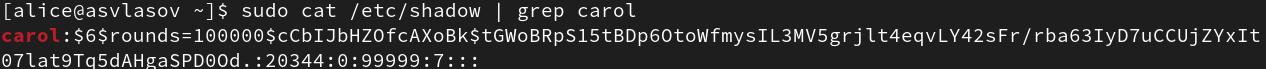
\includegraphics[width=0.7\textwidth,height=\textheight]{image/12.png}

}

\caption{Пароль}

\end{figure}%

Видим запись о пароле пользователя, 0 означает, что пароль бессрочный, и
должен быть использован за неделю до его изменения.

Меняем данные для пароля.

\begin{figure}

{\centering 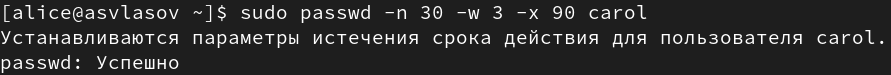
\includegraphics[width=0.7\textwidth,height=\textheight]{image/13.png}

}

\caption{Изм пароль}

\end{figure}%%
\begin{figure}

{\centering 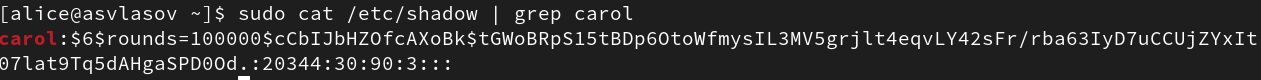
\includegraphics[width=0.7\textwidth,height=\textheight]{image/14.png}

}

\caption{Проверяем}

\end{figure}%

Смотрим, чтобы идентификатор alice был во всех файлах, а carol не во
всех.

\begin{figure}

{\centering 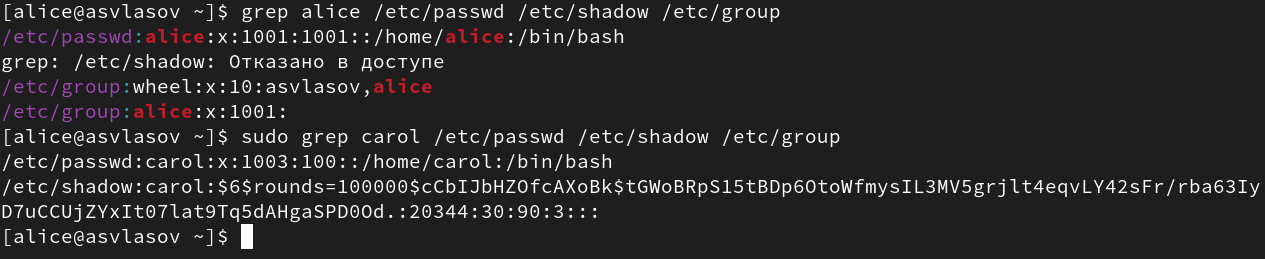
\includegraphics[width=0.7\textwidth,height=\textheight]{image/15.png}

}

\caption{Идентификатор}

\end{figure}%

Переходим к работе с группами.

Создаем две новых группы main и third.

\begin{figure}

{\centering 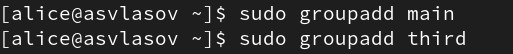
\includegraphics[width=0.7\textwidth,height=\textheight]{image/16.png}

}

\caption{Группы}

\end{figure}%

Добавляем пользователей в группы, и проверяем данные о пользователях.

\begin{figure}

{\centering 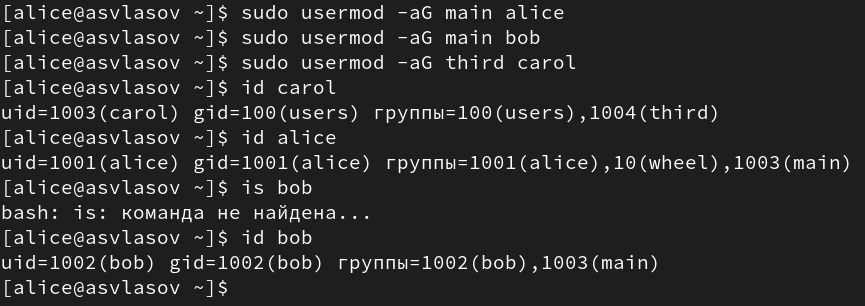
\includegraphics[width=0.7\textwidth,height=\textheight]{image/17.png}

}

\caption{Группы.}

\end{figure}%

Видим, что carol находится в группах users и third. Bob находится в
группах bob и main. A alice находится в группах main alice и группе
wheel с правами администратора.

\#Контрольные вопросы

\section{1. При помощи каких команд можно получить информацию о номере
(идентификаторе), назначенном пользователю Linux, о группах, в которые
включён
пользователь?}\label{ux43fux440ux438-ux43fux43eux43cux43eux449ux438-ux43aux430ux43aux438ux445-ux43aux43eux43cux430ux43dux434-ux43cux43eux436ux43dux43e-ux43fux43eux43bux443ux447ux438ux442ux44c-ux438ux43dux444ux43eux440ux43cux430ux446ux438ux44e-ux43e-ux43dux43eux43cux435ux440ux435-ux438ux434ux435ux43dux442ux438ux444ux438ux43aux430ux442ux43eux440ux435-ux43dux430ux437ux43dux430ux447ux435ux43dux43dux43eux43c-ux43fux43eux43bux44cux437ux43eux432ux430ux442ux435ux43bux44e-linux-ux43e-ux433ux440ux443ux43fux43fux430ux445-ux432-ux43aux43eux442ux43eux440ux44bux435-ux432ux43aux43bux44eux447ux451ux43d-ux43fux43eux43bux44cux437ux43eux432ux430ux442ux435ux43bux44c}

\begin{itemize}
\tightlist
\item
  id
\item
  id username
\item
  whoami
\item
  groups
\item
  groups username
\end{itemize}

\section{2. Какой UID имеет пользователь root? При помощи какой команды
можно узнать UID пользователя? Приведите
примеры.}\label{ux43aux430ux43aux43eux439-uid-ux438ux43cux435ux435ux442-ux43fux43eux43bux44cux437ux43eux432ux430ux442ux435ux43bux44c-root-ux43fux440ux438-ux43fux43eux43cux43eux449ux438-ux43aux430ux43aux43eux439-ux43aux43eux43cux430ux43dux434ux44b-ux43cux43eux436ux43dux43e-ux443ux437ux43dux430ux442ux44c-uid-ux43fux43eux43bux44cux437ux43eux432ux430ux442ux435ux43bux44f-ux43fux440ux438ux432ux435ux434ux438ux442ux435-ux43fux440ux438ux43cux435ux440ux44b.}

Пользователь root имеет UID 0.

Команды для определения UID: - id -u - id -u root - id -u username

\section{3. В чём состоит различие между командами su и
sudo?}\label{ux432-ux447ux451ux43c-ux441ux43eux441ux442ux43eux438ux442-ux440ux430ux437ux43bux438ux447ux438ux435-ux43cux435ux436ux434ux443-ux43aux43eux43cux430ux43dux434ux430ux43cux438-su-ux438-sudo}

\begin{itemize}
\tightlist
\item
  su - переключает на другого пользователя, требует пароль целевого
  пользователя
\item
  sudo - выполняет команду с привилегиями, требует пароль текущего
  пользователя
\end{itemize}

\section{4. В каком конфигурационном файле определяются параметры
sudo?}\label{ux432-ux43aux430ux43aux43eux43c-ux43aux43eux43dux444ux438ux433ux443ux440ux430ux446ux438ux43eux43dux43dux43eux43c-ux444ux430ux439ux43bux435-ux43eux43fux440ux435ux434ux435ux43bux44fux44eux442ux441ux44f-ux43fux430ux440ux430ux43cux435ux442ux440ux44b-sudo}

Файл /etc/sudoers

\section{5. Какую команду следует использовать для безопасного изменения
конфигурации
sudo?}\label{ux43aux430ux43aux443ux44e-ux43aux43eux43cux430ux43dux434ux443-ux441ux43bux435ux434ux443ux435ux442-ux438ux441ux43fux43eux43bux44cux437ux43eux432ux430ux442ux44c-ux434ux43bux44f-ux431ux435ux437ux43eux43fux430ux441ux43dux43eux433ux43e-ux438ux437ux43cux435ux43dux435ux43dux438ux44f-ux43aux43eux43dux444ux438ux433ux443ux440ux430ux446ux438ux438-sudo}

Команда sudo visudo

\section{6. Если вы хотите предоставить пользователю доступ ко всем
командам администрирования системы через sudo, членом какой группы он
должен
быть?}\label{ux435ux441ux43bux438-ux432ux44b-ux445ux43eux442ux438ux442ux435-ux43fux440ux435ux434ux43eux441ux442ux430ux432ux438ux442ux44c-ux43fux43eux43bux44cux437ux43eux432ux430ux442ux435ux43bux44e-ux434ux43eux441ux442ux443ux43f-ux43aux43e-ux432ux441ux435ux43c-ux43aux43eux43cux430ux43dux434ux430ux43c-ux430ux434ux43cux438ux43dux438ux441ux442ux440ux438ux440ux43eux432ux430ux43dux438ux44f-ux441ux438ux441ux442ux435ux43cux44b-ux447ux435ux440ux435ux437-sudo-ux447ux43bux435ux43dux43eux43c-ux43aux430ux43aux43eux439-ux433ux440ux443ux43fux43fux44b-ux43eux43d-ux434ux43eux43bux436ux435ux43d-ux431ux44bux442ux44c}

Группа sudo (Debian/Ubuntu) или wheel (RHEL/CentOS)

\section{7. Какие файлы/каталоги можно использовать для определения
параметров, которые будут использоваться при создании учётных записей
пользователей? Приведите примеры
настроек.}\label{ux43aux430ux43aux438ux435-ux444ux430ux439ux43bux44bux43aux430ux442ux430ux43bux43eux433ux438-ux43cux43eux436ux43dux43e-ux438ux441ux43fux43eux43bux44cux437ux43eux432ux430ux442ux44c-ux434ux43bux44f-ux43eux43fux440ux435ux434ux435ux43bux435ux43dux438ux44f-ux43fux430ux440ux430ux43cux435ux442ux440ux43eux432-ux43aux43eux442ux43eux440ux44bux435-ux431ux443ux434ux443ux442-ux438ux441ux43fux43eux43bux44cux437ux43eux432ux430ux442ux44cux441ux44f-ux43fux440ux438-ux441ux43eux437ux434ux430ux43dux438ux438-ux443ux447ux451ux442ux43dux44bux445-ux437ux430ux43fux438ux441ux435ux439-ux43fux43eux43bux44cux437ux43eux432ux430ux442ux435ux43bux435ux439-ux43fux440ux438ux432ux435ux434ux438ux442ux435-ux43fux440ux438ux43cux435ux440ux44b-ux43dux430ux441ux442ux440ux43eux435ux43a.}

Основные файлы: - /etc/login.defs - /etc/default/useradd - /etc/skel/

\section{8. Где хранится информация о первичной и дополнительных группах
пользователей ОС типа Linux? В отчёте приведите пояснение таких записей
для пользователя
alice.}\label{ux433ux434ux435-ux445ux440ux430ux43dux438ux442ux441ux44f-ux438ux43dux444ux43eux440ux43cux430ux446ux438ux44f-ux43e-ux43fux435ux440ux432ux438ux447ux43dux43eux439-ux438-ux434ux43eux43fux43eux43bux43dux438ux442ux435ux43bux44cux43dux44bux445-ux433ux440ux443ux43fux43fux430ux445-ux43fux43eux43bux44cux437ux43eux432ux430ux442ux435ux43bux435ux439-ux43eux441-ux442ux438ux43fux430-linux-ux432-ux43eux442ux447ux451ux442ux435-ux43fux440ux438ux432ux435ux434ux438ux442ux435-ux43fux43eux44fux441ux43dux435ux43dux438ux435-ux442ux430ux43aux438ux445-ux437ux430ux43fux438ux441ux435ux439-ux434ux43bux44f-ux43fux43eux43bux44cux437ux43eux432ux430ux442ux435ux43bux44f-alice.}

\begin{itemize}
\tightlist
\item
  /etc/passwd - первичная группа
\item
  /etc/group - дополнительные группы
\end{itemize}

\section{9. Какие команды вы можете использовать для изменения
информации о пароле пользователя (например о сроке действия
пароля)?}\label{ux43aux430ux43aux438ux435-ux43aux43eux43cux430ux43dux434ux44b-ux432ux44b-ux43cux43eux436ux435ux442ux435-ux438ux441ux43fux43eux43bux44cux437ux43eux432ux430ux442ux44c-ux434ux43bux44f-ux438ux437ux43cux435ux43dux435ux43dux438ux44f-ux438ux43dux444ux43eux440ux43cux430ux446ux438ux438-ux43e-ux43fux430ux440ux43eux43bux435-ux43fux43eux43bux44cux437ux43eux432ux430ux442ux435ux43bux44f-ux43dux430ux43fux440ux438ux43cux435ux440-ux43e-ux441ux440ux43eux43aux435-ux434ux435ux439ux441ux442ux432ux438ux44f-ux43fux430ux440ux43eux43bux44f}

\begin{itemize}
\tightlist
\item
  passwd
\item
  chage
\item
  usermod
\end{itemize}

\section{10. Какую команду следует использовать для прямого изменения
информации в файле /etc/group и
почему?}\label{ux43aux430ux43aux443ux44e-ux43aux43eux43cux430ux43dux434ux443-ux441ux43bux435ux434ux443ux435ux442-ux438ux441ux43fux43eux43bux44cux437ux43eux432ux430ux442ux44c-ux434ux43bux44f-ux43fux440ux44fux43cux43eux433ux43e-ux438ux437ux43cux435ux43dux435ux43dux438ux44f-ux438ux43dux444ux43eux440ux43cux430ux446ux438ux438-ux432-ux444ux430ux439ux43bux435-etcgroup-ux438-ux43fux43eux447ux435ux43cux443}

Команды: - groupadd - groupmod - groupdel - usermod

Прямое редактирование не рекомендуется из-за риска ошибок и повреждения
системных файлов.

\chapter{Выводы}\label{ux432ux44bux432ux43eux434ux44b}

Мы научились работать с пользователями и группами, задавать им права
пароли, и добавлять их в группы, ответили на контрольные вопросы.

\chapter*{Список
литературы}\label{ux441ux43fux438ux441ux43eux43a-ux43bux438ux442ux435ux440ux430ux442ux443ux440ux44b}
\addcontentsline{toc}{chapter}{Список литературы}

\printbibliography[heading=none]




\end{document}
